
\setcounter{chapter}{4}
\chapter{Sprint 3: Checkout API}
\minitoc %insert la minitoc
\graphicspath{{Chapter5/figures/}}

%\DoPToC
%==============================================================================
\pagestyle{fancy}
\fancyhf{}
\fancyhead[R]{\bfseries\rightmark}
\fancyfoot[R]{\thepage}
\renewcommand{\headrulewidth}{0.5pt}
\renewcommand{\footrulewidth}{0pt}
\renewcommand{\chaptermark}[1]{\markboth{\MakeUppercase{\chaptername~\thechapter. #1 }}{}}
\renewcommand{\sectionmark}[1]{\markright{\thechapter.\thesection~ #1}}


\begin{spacing}{1.2}

\section*{Introduction}
In this section, we will implement the tools needed for developers to be able to integrate Flouci in their websites. 

In order to make it portable in any existing e-commerce, we decided to implement it in pure javascript.
\section{Front end Integration}
In this section, we will implement the front end payment plugin that can can be integrated in any HTML code.
\subsection{User experience}
In the online payment, we faced a small issue regarding the payment experience, because the process is different from the mobile version. The online payments needs the developer to accept them.
So we decided to create the same QR code experience in mobile and only add a step to enter a six digits code in the browser.

\begin{figure}[H]\centering
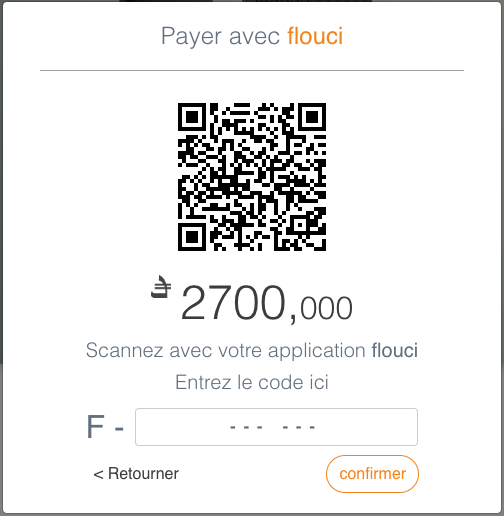
\includegraphics[scale=0.5]{payment_form.png}
\caption{Flouci payment Form}
\label{fig:register}
\end{figure}

\subsection{Code}
To create our front end form and make it easy to integrate, we created a web-pack project that bundles next generation javascript and css into one single javascript file.

\subsection{Integration}
After hosting the javascript file we can easily add the form to our project. The form will only require the public app key  and the amount.
The HTML code is listed in \ref{code:html}.
\begin{lstlisting}[rulecolor=\color{white}]
\end{lstlisting}
\begin{lstlisting}[label=code:html,caption=Flouci Integration Java,language=xml]
 <form id="myform" action="/handle_payment" method="post">
    <script
            src="https://developersdev.flouci.com/static/main.js"
            data-key="f6b5d0a5-e559-4acb-bcbb-a9e6ec9d788d"
            data-amount="2700000"
            data-name="Flouci Checkout"
            data-description="Flouci Data"

    </script>
  </form>
\end{lstlisting}


\section{Back end Integration}
After the user inputs the six digits code into the form, the form checks the validity of the payment and return a special key to the backend ( the action function inputed by the developer)

The developer then is only required to call an endpoint to accept the payment and then redirects the user to an other page depending on the payment result.

In the figure \ref{fig:flask} we show the code of a simple flask server with a Flouci integration that works with the HTML code listed in \ref{code:html}.
\begin{figure}[H]\centering
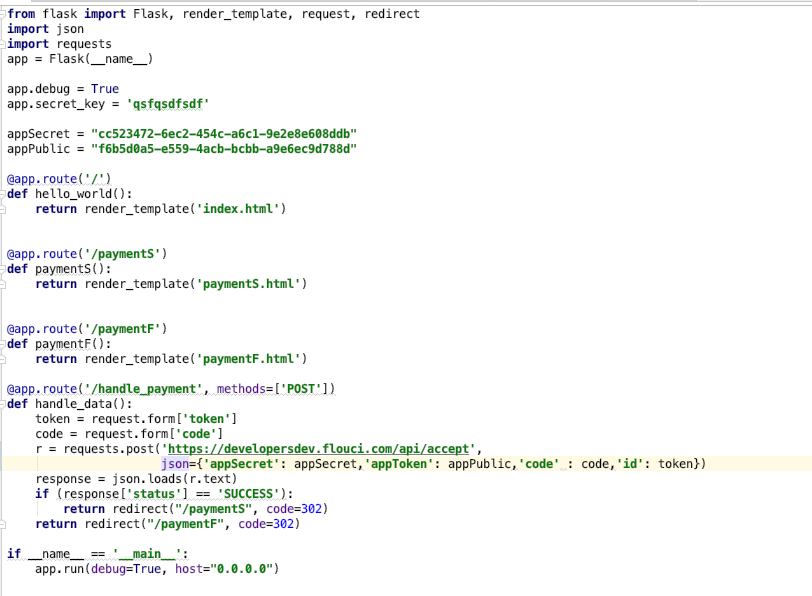
\includegraphics[scale=0.5]{flask.png}
\caption{Flouci payment Backend Integration}
\label{fig:flask}
\end{figure}
\section{Payment process}

\begin{figure}[H]\centering
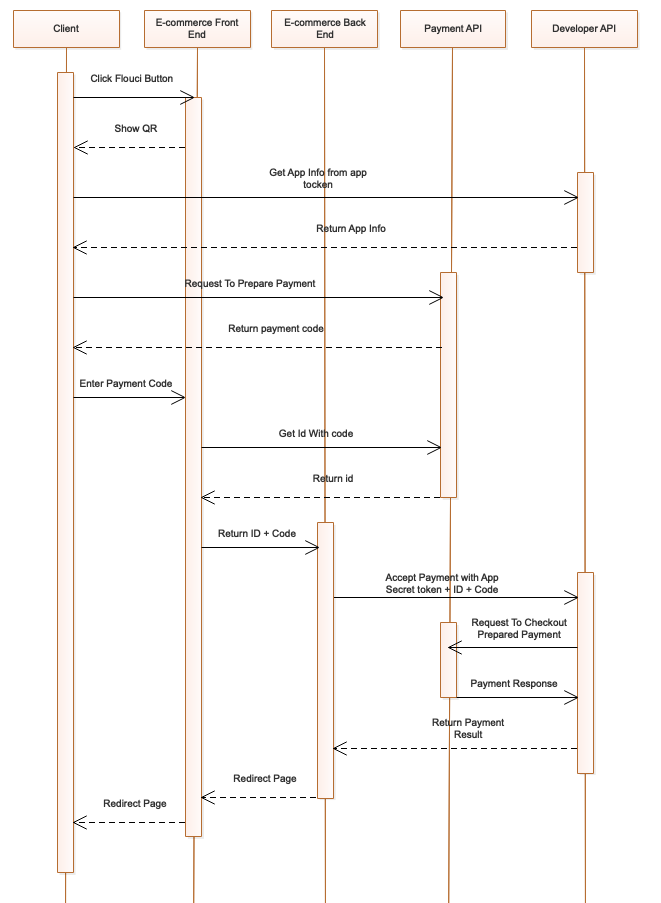
\includegraphics[scale=0.6]{Payment_Sequence_Diagram.png}
\caption{Flouci payment Backend Integration}
\label{fig:flask}
\end{figure}
\section*{Conclusion}
\end{spacing}
